%-------------------------------------------------------------------------------
% Evaluation. New text is wrapped in \textcolor{violet!85!black}{...} and prints in purple.
\section{\textcolor{violet!85!black}{Evaluation}}
\label{sec:evaluation}

\textcolor{red}{[OPEN: Setup: cluster and network, data size, YCSB workload and number of clients, replication factor, and what exactly the shaded migration window covers.]}

\subsection{\textcolor{violet!85!black}{Migration under failures}}
\label{sec:eval-failures}

\begin{figure*}[t]
  \centering
  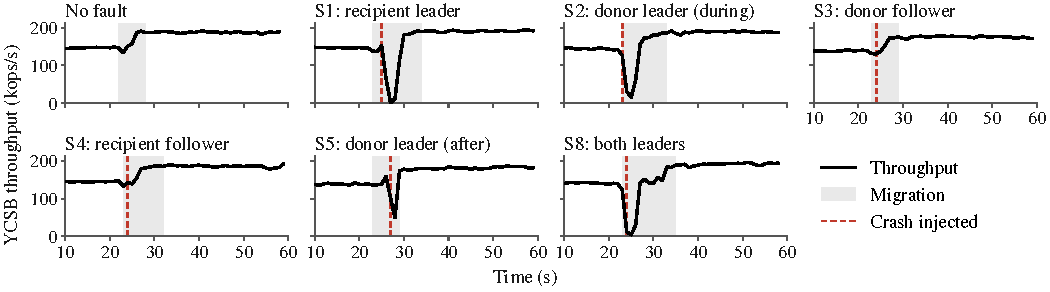
\includegraphics[width=\textwidth]{figs/all_scenarios_throughput.pdf}
  \caption{\textcolor{violet!85!black}{YCSB throughput during a migration with injected crashes. The shaded band is the migration, and the dashed line marks the crash.}}
  \label{fig:eval-failures}
\end{figure*}

\textcolor{violet!85!black}{We migrate slots between shard groups while a YCSB workload runs, and we crash one or two nodes during the migration.
Fig.~\ref{fig:eval-failures} shows the throughput of the cluster in seven scenarios.
In every scenario, the migration completes and throughput reaches the same level as in the run without faults.}

\paragraph{\textcolor{violet!85!black}{No fault.}}
\textcolor{violet!85!black}{The migration takes about 6\,s and causes only a small dip in throughput.
Once it completes, throughput rises from about 145 to about 190\,kops/s, an increase of about 30\%.}
\textcolor{red}{[OPEN: State where the gain comes from, e.g., the recipient taking over part of the load.]}

\paragraph{\textcolor{violet!85!black}{Follower crashes.}}
\textcolor{violet!85!black}{A crash of a donor follower (S3) or of a recipient follower (S4) causes no visible drop in throughput.
With a crashed recipient follower, the migration takes about 9\,s instead of 6\,s.}
\textcolor{red}{[OPEN: Confirm that the extra time in S4 is chain repair (Section~\ref{sec:failure-handling}).]}

\paragraph{\textcolor{violet!85!black}{Leader crashes.}}
\textcolor{violet!85!black}{When the recipient leader crashes during the migration (S1), throughput drops to almost zero for about 2\,s and is back within about 5\,s of the crash.
When the donor leader crashes during the migration (S2), throughput drops to about 15\,kops/s and recovers within about 4\,s.
When the donor leader crashes at the end of the migration (S5), throughput dips to about 50\,kops/s for about 1\,s.
When both leaders crash (S8), throughput drops to almost zero, returns to its level before the migration within about 4\,s, and the migration completes about 11\,s after the crash.}
\textcolor{red}{[OPEN: Explain why the throughput of the whole cluster drops, not only that of the migrating slots, and relate the length of the drop to the election timeout.]}

\paragraph{\textcolor{violet!85!black}{Correctness.}}
\textcolor{violet!85!black}{We also check that the migration preserves the data in every scenario.
During each run, the clients record every write that the store acknowledges.
After the migration completes, we read every key back and compare the migrated slots across the replicas of the recipient shard group.
In all seven scenarios, no acknowledged write was lost, no deleted key reappeared, and all replicas of the recipient held identical data for the migrated slots.}
\textcolor{red}{[OPEN: Fill in: what exactly was checked and how (read-back of acknowledged writes, per-slot digest across replicas, linearizability checker?), the number of runs per scenario, and the number of keys or operations checked. Adjust the sentence above to what was actually verified.]}

\textcolor{red}{[OPEN: Scenarios S6 and S7 are not shown: renumber, or say why they are omitted. Add tail latency (p99) for the same runs.]}
